\documentclass{article}
\usepackage{amsmath, amssymb, amsfonts, amsthm}
\usepackage[margin=1in]{geometry}
\usepackage{fancyhdr}
\usepackage[final]{pdfpages}
\usepackage[makeroom]{cancel}
\usepackage{enumitem}
\usepackage[flushleft]{threeparttable}
\usepackage[normalem]{ulem} 
\usepackage{hyperref} % include url

\newcommand{\lecture}[3]{
   \pagestyle{myheadings}
   \thispagestyle{plain}
   \newpage
   \setcounter{page}{1}
   \noindent
   \begin{center}
   \framebox{
      \vbox{\vspace{2mm}
      \hbox to 6.28in {Rensselaer Polytechnic Institute \hfill CSCI-4968: ML and Optimization}
        \vspace{5mm}
        \hbox to 6.28in { {\Large \hfill #1 \hfill} }
        \vspace{2mm}
         \hbox to 6.28in { {\hfill \ \ \ \ \ #3 \hfill} }
        \vspace{2mm}
         \hbox to 6.28in { {\footnotesize{\url{https://github.com/Xinshi0726/SDP-Relxations-With-Applications}} \hfill April 2023}}
        % \vspace{2mm}
      }
   }
   \end{center}
   \markboth{Lecture: #1: #2}{Lecture: #1: #2}
}

\begin{document}

\lecture{Semidefinite Programming}{}{Applications in approximating NP-Complete problems \& Matrix Completetion}

\section{Motivation}
Linear programming is a common constrained optimization problems with uses in several fields including math, computer science, economics, and buisness.
% The power and ubiquity of linear programming comes 
% from the fact that it can solve a wide host of linear constrained optimization problems.
Seveal real world problems can be modelled as a set of linear contraints, making linear programming a ubiquitous construct.
% One use case arises in manufacturing. Given a set of products, how much of each kind should be produced to either minimize cost or maximize profits?
% Linear programming is a general approach of taking a constrained linear optimization problem into a form where a solution can easily be found.
% linear programming usable in a large variety of problems such as
We are able to find solutions to a linear program in polynomial time.

% Not only can solutions can be found, but they can also be found quite quickly.
% https://arxiv.org/abs/1810.07896
Semidefinite programming (SDP) expands on the ideas used within linear programming and generalizes them so that they can be applied to more problems, including nonlinear optimization problems.
% Instead of being able to control single variables, we are able to select for an entire matrix, with whole matricies of constraints.
SDPs are widely used for combinatorial optimization - a class of problems that are of abundance in network science.
The notorious NP-Hard problems can be approximated quite well with SDPs.
The flexibility and speed of finding solutions of what can be represented as a SDP problem is what gives it its power. 

% We will go over how to relax a classic NP-Complete problem, the Travelling Salesman into a semidefinite program, 
% and how it can be used to fill in the data given a sample of a low rank. 
% We then provide guide on how it can be used to approximate another NP-Complete Problem, Max Cut.
We will go over how to approximaate a classic NP-Complete problem, the Travelling Salesman 
and how it can be used to complete partially filled matricies of low-rank.
We then provide guide on how it can be used to approximate another NP-Complete Problem, Max Cut.

\section{Semidefinite Programming}  % objective functions

\subsection{Overview of Linear Programming}
To give background on semi-definite programming, we begin with a brief recap of linear programming.
Suppose that you have control over a set of variables and you are attempting to find a selection for each of these variables such that some linear combination is either maximized or minimized.
Formally we can write this out as the following. Suppose that we have \( n \) variables that we have control over. This is represented as:
\[
\vec{x} = \begin{bmatrix} x_1 \\ x_2 \\ \vdots \\ x_n \end{bmatrix}
\]

Say for each of these \( n \) variables has an associated coefficient \( \vec{c} = \begin{bmatrix} c_1, c_2, ..., c_n  \end{bmatrix}^\top \).
We would like to find \( \vec{x} \) such that \( \vec{c} \cdot \vec{x} \) is minimized

This problem is made trivial by setting \( \vec{x} \) to be arbitrarily large or small value depending on the optimization direction.
The solution becomes more meaningful if the domain of each variable is constrainted.

% \begin{align*}
%   \begin{array}{ll@{}ll}
%   \min  & \vec{c} \cdot \vec{x}
%   \end{array}
% \end{align*}

Suppose we have vectors \( \vec{a}_i \) and \( \vec{b} \) in $\mathbb{R}^n$.
Extending the above idea to a system of equations, we would like to find \( \vec{x} \) such that
\begin{align*}
\vec{a}_1 \cdot \vec{x} &\leq b_1 \\
\vec{a}_2 \cdot \vec{x} &\leq b_2 \\
& \vdots  \\
\vec{a}_n \cdot \vec{x} &\leq b_n \\
\end{align*}

\newpage

Graphically, each constraint creates a \emph{half-space}. 
The intersection of the halfspaces (the white space) is our solution set. 
Our goal is the find the value of \( \vec{x} \) within this white space such that our objective function is minimized.\\
\vspace{-1.3em}
\begin{figure}[ht]
  \centering
  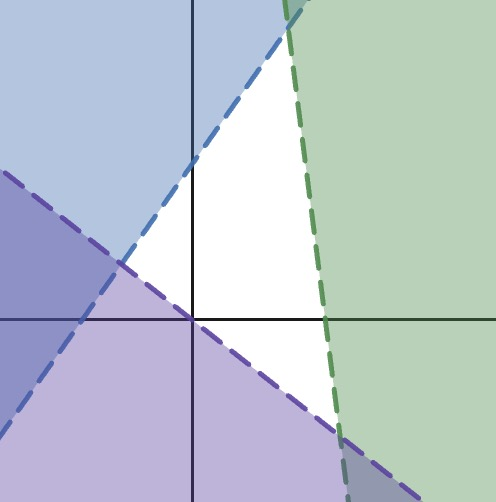
\includegraphics[scale=.2]{assets/half_space.jpg}  
  \caption{Graphical representation of linear inequalties}
\end{figure}

Instead of dealing with inequalities we can transform our constraints into equalities.
Suppose one of the constraints is \( \vec{a}_{k} \cdot \vec{x} \leq b_{k} \).
We can introduce a new variable \( x_{n + 1} \) such that \( x_{n + 1} \geq 0 \) and then take our constraint so that it is now \( \vec{a}_k \cdot \vec{x} + x_{n + 1} = b_k \).
Following this we can gather our \( \vec{a}_i \) vectors into a single matrix.
Let $\mathbf{A} = [\vec{a_1}^\top \cdots \vec{a_n}^\top]$ so that our constraint becomes:
\[
\mathbf{A} \vec{x} = \vec{b}
\]

Additionally we would like \( \vec{x} \) to be nonnegative.
\[ \vec{x} \geq 0 \]. 

In summary, linear programming is a technique used to find an optimal solution, \( \vec{x} \) to a linear objective function when we are given a set of linear constraints.
\begin{align*}
  \begin{array}{ll@{}ll}
    \text{minimize}   & \vec{c} \cdot \vec{x}& \\
    \text{subject to} & \mathbf{A} \vec{x} &=  \vec{b} \\
                      & \vec{x} &\geq 0 \\
    \end{array}
\end{align*}

We note that our constraints form a convex set.
Thus, linear programming is a subset of a convex optimization problem.
Finding a solution to an instance of linear programming can be done with a variety of algorithms including the \emph{simplex algorithm}.

\subsection{Formalization of Semidefinite Programming}
With linear programming, we optimize over  \( n \) variables. Now, suppose we have \( n^2 \) elements. 
Thus instead of finding an optimal \( \vec{x} \in \mathbb{R} \), we'd like to find an optimal 
\( \mathbf{X} \in \mathbb{R}^{n \times n} \).
A common intrepretation of positivity for matricies is \emph{positive semi-definite} (PSD). 
Positive semidefinite matrices are symmetric and when operated upon, will output a positive number. That is, for 
arbitrary $\vec{v}$, $\vec{v}^\top\mathbf{X}\vec{v} > 0$.
We constraint \( \mathbf{X} \) to be positive semi-definite or \( \mathbf{X} \succeq 0 \).
Let \( \mathbf{C} \in \mathbb{R}^{n \times n}\) be a matrix where $c_{i,j}$ is the coefficient corresponding 
to the \( x_{i, j} \) variable.
Generalizing ideas introduced in linear programming, we have
\begin{align*}
  \begin{array}{ll@{}ll}
  \min & \displaystyle\sum\limits_{i=1}^{n}\sum\limits_{j=1}^{n} x_{i, j} c_{i , j} &\\
  \text{s.t} & \mathbf{X} \succeq 0 
  \end{array}
\end{align*}

We introduce the Frobenius inner product which is the sum of element wise multiplication on vectors:
% is simply taking the sum of all elements after doing element wise multiplication on two matricies \( \mathbf{C} \) and \( \mathbf{X} \) with the same shape.
\[
  \langle \mathbf{C}, \mathbf{X} \rangle_{\mathrm{F}} = \sum_{i = 1}^n \sum_{j = 1}^n \mathbf{C}_{i, j} \mathbf{X}_{i, j}
\]

Of important note is the fact that \( \langle \mathbf{C}, \mathbf{X} \rangle_{\mathrm{F}} = \text{trace}(\mathbf{C}^\top \mathbf{X}) \) where \( \text{trace} \) is the sum of the diagonal terms for a matrix. Calculating the \( \text{trace} \) of the matrix multiplication is not as efficient as the Frobenius inner product but the notation comes up quite frequently within the literature making it important to know.

Returning back to our formalization of SDP, we note that with more variables comes with more constraints. Suppose that we have \( m \) equations to satisfy. For each equation we have a matrix \( \mathbf{A}_i \) and a scalar value \( b_i \) defining our constraint. Then for a given constraint we have:
\[
\langle \mathbf{A}_i, \mathbf{X} \rangle_{\mathrm{F}} = b_i
\]
This is all that is needed for SDP. We can write this out formally as:

\begin{align*}
  \begin{array}{ll@{}ll}
  \min              & \langle \mathbf{C}, \mathbf{X} \rangle_{\mathrm{F}}                   & \\
  \text{subject to} & \langle \mathbf{A}_i, \mathbf{X} \rangle_{\mathrm{F}} &= b_i       & i=1 ,\dots, m\\
                    & \mathbf{X}                      &\succeq 0
  \end{array}
\end{align*}

The parallels between semidefinite programming and linear programming should be quite apparent.
In many ways, semidefinite programming is linear programming with more variables and more constraints.
\subsection{Semidefinite Programming Duality}
It won't be explained in depth here, but it is also useful to know what the dual of SDP looks like. From before we know that SDP is defined as

\begin{align*}
  \begin{array}{ll@{}ll}
  \min              & \langle \mathbf{C}, \mathbf{X} \rangle_{\mathrm{F}}                   & \\
  \text{subject to} & \langle \mathbf{A}_i, \mathbf{X} \rangle_{\mathrm{F}} &= b_i       & i=1 ,\dots, m\\
                    & \mathbf{X}                      &\succeq 0
  \end{array}
\end{align*}
We note that we have to satisfy \( m \) equations. Then the dual is defined as:
\begin{align*}
  \begin{array}{ll@{}ll}
    \max              & \vec{z} \cdot \vec{b}                              & \\
    \text{such that}  & \sum_{i=1}^m z_i \mathbf{A}_{i} + \mathbf{S} &= \mathbf{C} \\
                      & \mathbf{S}                      &\succeq 0
  \end{array}
\end{align*}

Where we are trying to find a set of scalar values \( z_1, z_2, \ldots, z_m \) such that the dot product \( \vec{z} \cdot \vec{b} \) is maximized while also satisfying that \( \sum_{i=1}^m z_i \mathbf{A}_{i} + \mathbf{S} = \mathbf{C} \) where \( \mathbf{A}_i \) and \( \mathbf{C} \) are from before.
We know that \( \mathbf{S} \succeq 0 \) which gives us the slightly more intuitive and equivalent optimization problem:

\begin{align*}
  \begin{array}{ll@{}ll}
    \max              & \vec{z} \cdot \vec{b}                              & \\
    \text{such that}  & \mathbf{C} - \sum_{i=1}^m z_i \mathbf{A}_{i}  &\succeq 0 \\
  \end{array}
\end{align*}

\subsection{Semidefinite Programming Running Time}
The only reason why SDP would be useful at all in the first place is if it was able to be solved in polynomial time.
There are a variety of algorithms that can solve SDPs. 
One such algorithm is Alizadeh's interior point method \cite{Arora} which runs in:
\[ \tilde{O}(n^{3.5}) \]

\section{Travelling Salesman Relaxation}   % objective functions
Imagine you are prospective student touring RPI. You have a list of buildings you want to visit.
You have on hand the distance between each pair of buildings. 
Is it possible to find a path such that each buidling is visited exactly once? 
If so, what is the shortest possible distance you will need to travel. 
Since you toruing the college, it is likely you have some method of transportation to came from and need to come back to . 
We have the added constraint that you start at the parking lot and will need to come back to the parking lot.
This is know as the euclidean travelling salesman. We say euclidean as the distances between two points are distances is the 
two norm. 
% One sentence Goal
As our goal is to find an \emph{efficient} route, we will be satisfied with an approximation. 
Or a series of buidlings to visit that is close the optimal.
\subsection{Relaxation For Traveling Salesman}

% First desribe what the hamiltonian cycle is
% how the matrix X encodes a  cycle

% Desired or "perfect" SDP

% SDP relaxation

Let $C \in \mathbb{R}^{n \times n}$ denote the matrix of edge costs. Let $J$ denote the all-ones matrix, and $e$ denote the all-ones vector.
\begin{equation*}
\begin{aligned}
& {\text{minimize}}
& & \frac{1}{2}\text{trace}(CX) \\
& \text{subject to}
& & Xe = 2e \\
&&& X_{ii} = 0, \quad i = 1,\ldots,n\\
&&& 0 \leq X_{ij} \leq 1, \quad i,j = 1,\ldots,n \\
&&& 2I - X + (2-2\cos\left(\frac{2\pi}{n}\right))(J-I) \succeq 0 \\
&&& X \text{ is a real, symmetric } n \times n \text{ matrix}.
\end{aligned}
\end{equation*}

\noindent X is a fractional adjacency matrix, meaning for $e = \{i, j\}$, $x_{ij} = x_{ji}$ is the proportion of edge $e$ used.
\subsubsection{Explanation For Each Constraint}
\begin{enumerate}
    \item $Xe = 2e$ means the sum of each row in the adjacency matrix should equal to 2. This is trivial as we have an origin and destination as \ref{fig:degrees} suggests. 
    \item $X_{ii} = 0$ is trivial as the distance from a city to itself is always 0.
    \item $0 \leq X_{ij} \leq 1, \quad i,j = 1,\ldots,n$ is a relaxation that does not enforce an exact solution. i.e, we can have a fractional value for each edge.
    \item $2I - X + (2-2\cos\left(\frac{2\pi}{n}\right))(J-I) \succeq 0$ is the tricky part of the formulation. An understanding is not required but an explanation is given below.
\end{enumerate}
The constraint $2I - X + (2-2\cos\left(\frac{2\pi}{n}\right))(J-I) \succeq 0$ is related to the idea of graph spectrum, Laplacian of Hamiltonian cycle, and algebraic connectivity. Here are some facts needed in order to understand the meaning of the constraint:
\begin{enumerate}
    \item Let $ G_C = (V, E, C)$ denote a C-edge-weighted graph with nonegative edge values, Laplacian $L(G_C)$ is defined as $L(G_C) = diag(r_1,...,r_n)-C$, where $r_i$ is the sum of the i-th row of C.
    \item $L(G_C)$ is symmetric, positive semidefinite with the smallest eigenvalue $\lambda_1$ = 0 and the corresponding eigenvector $e$.
    \item The algebraic connectivity $\alpha(G_C)$ is the second smallest eigenvalue of $L(G_C)$. There are two main properties: $(1).\alpha(G_C) = \underset{x \in S}{min}x^TL(G_C)x$ \quad $(2).\alpha(G_C) \geq 0$, and $\alpha(G_C) > 0$ iff $G_C$ is connected. 
    \item Algebraic connectivity of a Hamiltonian circuit is well known in the theory of graph spectra. The Laplacian of a circuit with n vertices has the spectrum $$2-2 cos(2\pi j/n), j = 1,...,n$$
    and the second smallest eigenvalue is obtained for $j = 1$ and $j = n-1$, i.e. $\lambda_2 = \lambda_3 = 2-2cos(2\pi/n)$. This value will be denoted by $h_n$, i.e. $h_n = 2-2cos(2\pi/n)$.
\end{enumerate}
The constraint is making sure weighted graph corresponding to X (as a weighted adjacency matrix) is at least as connected as a cycle graph, with respect to algebraic connectivity. $2I-x$ gives us the Laplacian matrix corresponding to the weighted graph according to entries of x. $J$ makes sure we ignore trivial eigenvalues of Laplacian $\lambda = 0$. $2-2cos(2\pi/n)$ makes sure that the non-trivial eigenvalues is greater than or equal to the second smallest eigenvalue of a connected Hamiltonian Cycle.
\begin{figure}[!ht]
    \centering
    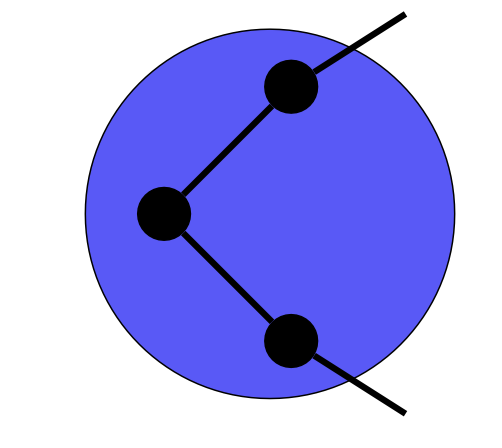
\includegraphics{assets/degrees.png}
    \caption{Caption: A node in the Hamiltonian Cycle}
    \label{fig:degrees}
\end{figure}

\subsection{Experiments}

\subsubsection{Integrality Gap And Running Time}
\begin{table}[!ht]
\begin{threeparttable}
\caption{SDP/Brute Force Methods Comparison}
\begin{tabular}{|l|l|l|l|l|l|l|}
\hline
\# Of Nodes & SDP  Time & BF Time  & SDP Objective Value & BF Objective Value & Integrity Gap & Time Ratio \\
\hline
10          & 0.7101    & 0.0156   & 53224.4854          & 53228.3976         & 0.9999        & 45.519     \\
15          & 0.6776    & 0.8224   & 65753.5934          & 67299.5625         & 0.9770        & 0.8239     \\
20          & 1.2271    & 97.2059  & 69558.9865          & 76199.4928         & 0.9129        & 0.0126     \\
21          & 1.3689    & 266.7778 & 73969.6527          & 77373.6362         & 0.9560        & 0.0051     \\
22          & 5.4774    & 657.7847 & 66459.7265          & 68245.9576         & 0.9738        & 0.0083     \\
 \hline
\end{tabular}
\begin{tablenotes}
      \small
      \item 1. BF denotes the brute force method and was implemented using dynamic programming
      \item 2. Integrity Gap is the ratio between SDP Objective Value and BF Objective Value
    \end{tablenotes}
\end{threeparttable}
\end{table}

Our SDP solver grows much more slowly as compared to the brute force approch. The objective values of 
SDP is lower then the true optimal solution (as indidcated in BF Objective Value). For our small examples, we
are able to find a good lower bound. 
\subsubsection{Visualization}
Our SDP relaxation will yield an objective value respresentive of the lower bound. 
The final $\mathbf{X}$ matrix is a fractional adjacency matrix. As such, for an edge with a high value,
it can be intrpreted as a being a high probability of being an edge in the Hamiltonian cycle.
To find the Hamiltonian cycle, we set the edge that has value greater   than or equal to the $3^{rd}$ largest value in that row to 1 and else 0 to find the adjacency matrix.
Then we use the adjacency matrix and coordinates of points to plot the results.
\begin{figure}[!ht]
    \centering
    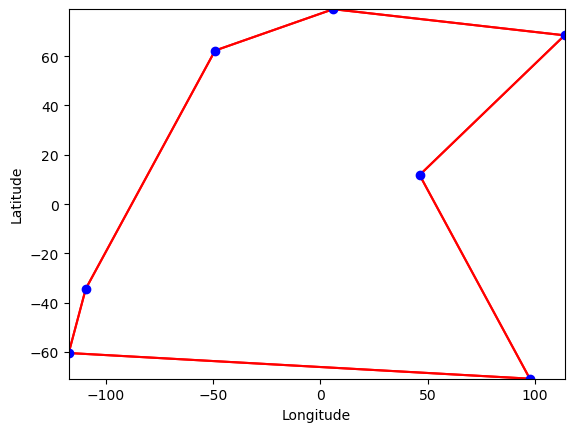
\includegraphics[width=0.3\textwidth]{assets/tsp7.png}
    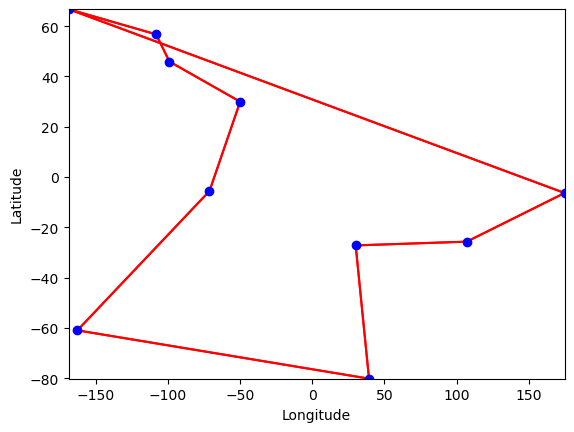
\includegraphics[width=0.3\textwidth]{assets/tsp-10.png}
    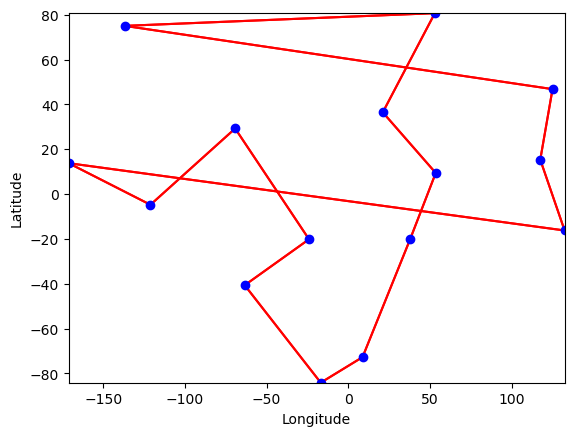
\includegraphics[width=0.3\textwidth]{assets/tsp-15-works.png}
    \caption{Sets of the Problems that SDP Relaxation is able to find a reasonable solution}
    \label{fig:TSP Graph}
\end{figure}
\begin{figure}[!ht]
    \centering
    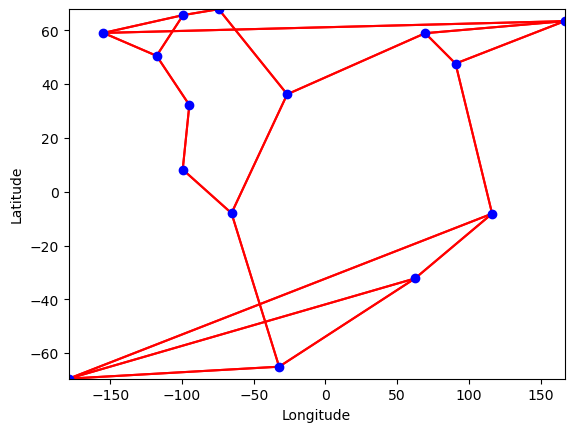
\includegraphics[width=0.3\textwidth]{assets/tsp-15.png}
    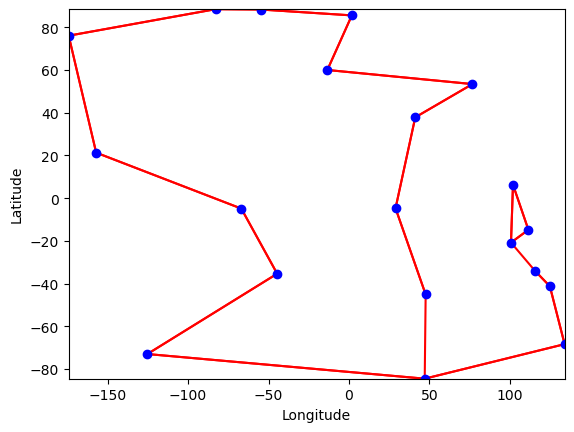
\includegraphics[width=0.3\textwidth]{assets/tsp-20.png}
    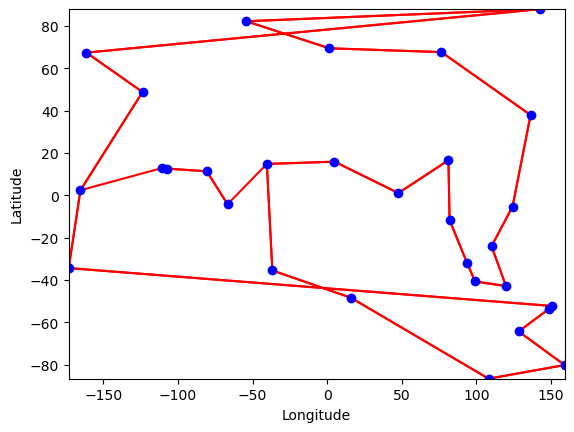
\includegraphics[width=0.3\textwidth]{assets/tsp-30.png}
    \caption{Sets of the Problems that SDP Relaxation is unable to find a resonable solution}
    \label{fig:TSP Graph 2}
\end{figure}


We find that it is easy to break the Hamiltonian cycle, espically as the the number of nodes increases.

% \section{Discussion}

% - can we prove the runtime
% - can we prove how good of a lower bound we have?
% - what are some easy things to prove?
% \subsection{Scope and limitations}

\newpage 
\section{Matrix Completetion}

% Analyzing data in high-dime
% high dimensional data. Fortunately, these data lie in low dimensional subspaces

% While many data of interest, such as images, genome, customers' preference rankings, are often presented in high dimension,
% it is often the case that these high dimensional data lie in a low dimensional subspace. 
% This is true of images as well. 

% Suppose we have low rank matrix
% -- go through motivation of low rank matricies
% -- introduce idea of images

Suppose we have a incomplete sampling of some data. Are we able to fill in the missing values? 
When dealing with low dimensional data, given a representative sampling, it is possible to recover the missing entires. 
Low rank matrices are special in that they have a sparse set of singular values. This means much 
of the data can be described in few singular vectors. 
Singular vectors describes the variance of the data. Singular vectors associated with larger singular values
retains a larger variance, while singular vectors of the smaller singular values do not hold as much value. 
% , which describe the variance of the data.

% Low rank matrices can be compressed quite well as they can usually be decomposed 
% into a combination of simplier matrices. One such decomposition  is singular value decompostion. 

We will walk through how to formulate a low rank matrix completion problem into a semidefinite program problem.
We then show how it performs with some low rank images. 

\subsection{Relaxation}

Suppose we have a low rank matrix $\mathbf{M}$. We have a set of location $\Omega$ describing
our sampling. That is, if $(i,j) \in \Omega$, we observe entry $M_{ij}$. Given $\mathbf{M}$ is low rank, 
it seems resonable that we would like to solve the following optimization problem

\begin{equation*}
  \begin{aligned}
  & {\text{minimize}}
  & & \text{rank}(\mathbf{X}) \\[1pt]
  & \text{subject to}
  & & X_{ij} = M_{ij} \quad (i,j) \in \Omega\\[1pt]
  &&& \mathbf{X} \in \mathbb{R}^{n \times n}
  \end{aligned}
\end{equation*}

We make the assumption that $|\Omega|$ is sufficiently large and its entries are uniformly distributed throughout 
$\mathbf{X}$.
This makes it reasonable to assume there exists only one low rank matrix under the constraints. 
However, the rank is not a convex. The above problem is very hard to solve. In fact, it is NP-hard. 

We instead rely on the nuclear norm, a close approximation of the rank. The nuclear norm of a matrix $\mathbf{X}$ is defined as the sum of 
the singular values.
\[
\lVert \mathbf{X} \rVert_* = \sum_{k=1}^n \sigma_k ({\mathbf{X}})  
\]

For a symmetric positive semi-definite (SPSD) matricies, the nuclear norm is equal to the trace. 
However, the matrix we would like to recover, $\mathbf{M}$ is not necessarily SPSD.
As this is quite the constraint on the input data, we augment $\mathbf{X}$ with two matrices 
$\mathbf{W}_1$ and $\mathbf{W}_2$ to create a SPSD matrix. Solving the following will yield an 
$\mathbf{X}$ that recovers $\mathbf{M}$ given the entries specified by $\Omega$.

\begin{equation*}
  \begin{aligned}
  & {\text{minimize}}
  & & \text{trace}(\mathbf{W}_1) + \text{trace}(\mathbf{W}_2) \\[1pt]
  & \text{subject to}
  & & X_{ij} = M_{ij} \quad (i,j) \in \Omega\\[1pt]
  &&& \begin{bmatrix} 
    \mathbf{W}_1 & \mathbf{X} \\
    \mathbf{X}^\top & \mathbf{W}_2
  \end{bmatrix} \succeq 0 
  \end{aligned}
\end{equation*}


% We note for for $\mathbf{X}$ to reprensent 
% \[ 
% m \geq Cn^{6/5}rlogn
% \] 
\subsection{Image recovery}

Suppose you have a corrupted image. You have knowledge which pixels remains uncorrupted. Can we use matrix completion to
fill in the corrrupted portion? 

We test how matrix completion work with the Fashion-MNIST data. Each image is a 28 $\times$ 28 grayscale image. 
We corrupt the images by masking a percentage of the pixels. Next, we used the relaxation described above to 
recover the original image. 

\begin{figure}[htb]
  \centering
  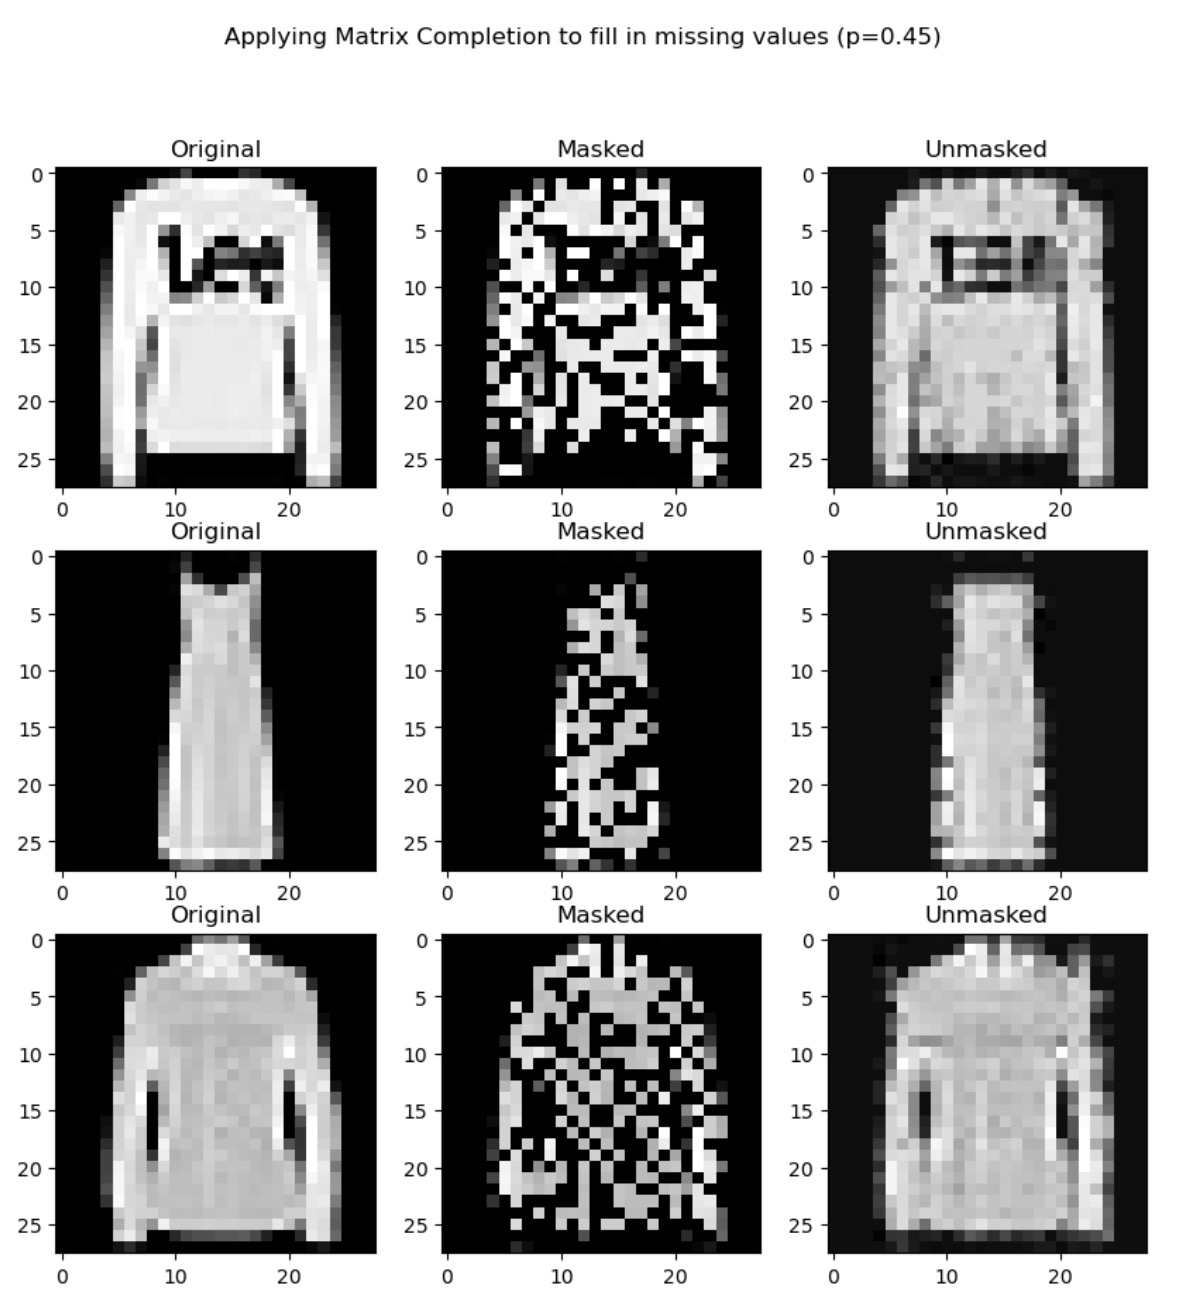
\includegraphics[scale=.25]{assets/mc-r1.jpg}
\end{figure}

We find that we are still able to recover a good representation of the original given $55\%$ of the data (remove $p = 45\%$)
We note for large images, a smaller percentage data is needed to recover to $\mathbb{M}$.
For smaller matrices, each entry is weighted more heaviely. Errors would also be magnified. 

\newpage
\section{Appendix}
\subsection{Problem Set}
We will now give one application of semidefinite programming in approximating an NP-Hard problem.
We will first formalize the SDP and then use to find the approximation.

Consider the max-cut problem where for graph \( G \) the goal is to split the vertices into two disjoint sets \( S \) and \( \overline{S} \) such that the sum of the edges between the two sets is maximum.
Thus we know that \( S \cup \overline{S} = V(G) \) and \( e(i, j) \) is the weight of the edge between vertex \( v_i \) and vertex \( v_j \).
Thus our optimization problem is:
\[
  \max \sum \{ e(i, j): v_i \in S \text{ and } v_j \in \overline{S} \}
\]
We will collect all our edge weights into matrix \( \mathbf{W} \) where \( w_{i, j} \) is the edge weight between vertex \( v_i \) and \( v_j \).

We will work our way towards a formalization of SDP.
\subsubsection{Question 1.}
For all of our vertices we have a corresponding variable \( x_i \) such that:
\begin{gather*}
x_i \in \{ -1, 1 \} \\
\text{if } x_i \in S \text{ then } x_i = 1 \\
\text{if } x_i \in \overline{S} \text{ then } x_i = -1 \\
\end{gather*}
Then for two vertices \( v_i, v_j \in V(G) \) what is the inuition behind the following equation:
\[
w_{i, j}(1 - x_i x_j)
\]
Answer: If \( v_i \) and \( v_j \) are in the same set the above equation will be zero otherwise \( w_{i, j} \) will be returned. The weight will only get returned if the edge between \( v_i \) and \( v_j \) is a cut edge for the sets \( S \) and \( \overline{S} \).

\subsubsection{Question 2.}
How can we turn \( x_i x_j \) from above into a matrix given that \( \vec{x} = [x_1, x_2, \ldots, x_n] \). This matrix should be square with the number of rows equal to the number of vertices in our graph. \( \mathbf{X}_{i, j} = x_i x_j \):
Answer:\( \mathbf{X} = \vec{x} \vec{x}^\top \)

\subsubsection{Question 3.}
What can you say about the values on the diagonal of \( \mathbf{X} \)? Is \( \mathbf{X} \) symmetric?

\subsubsection{Question 4.}
Before we found that our optimization problem was:
\[
  \max \sum \{ e(i, j): v_i \in S \text{ and } v_j \in \overline{S} \}
\]
And in question 1. we found that for a single vertex pair we have:
\[
w_{i, j}(1 - x_i x_j)
\]
How can we rewrite our optimization problem to account for all vertex pairs using \( \mathbf{X} \) and \( \mathbf{W} \) and the Frobenius inner product.
Ensure that in your solution that no edge is counted twice:

Answer:
\begin{align*}
 &= \max \frac{1}{2} \left (\sum_{i = 1}^n \sum_{j = 1}^n[ w_{i, j}(1 - x_i x_j) ] \right)\\
 &= \max  \sum_{i = 1}^n \sum_{j = 1}^n[ w_{i, j} - w_{i, j} x_i x_j ]\\
 &= \max \frac{1}{2} \left ( \sum_{i = 1}^n \sum_{j = 1}^n[w_{i, j}] - \langle \mathbf{W}, \mathbf{X} \rangle_{\mathrm{F}} \right )
\end{align*}

Since 
The \( \frac{1}{2} \) comes from the fact that \( \mathbf{X} \) and \( \mathbf{W} \) are symmetric and thus each cut edge is counted twice.

\subsubsection{Question 5.}
We have formalized the value that we want to maximize in the previous question.
One of our constraints for SDP is that \( \mathbf{X} \) has to SPSD.
Thus we know that \( \mathbf{X} \succeq 0 \).
Currently our constraints are that for \( x_{i, j} \in \mathbf{X} \) that \( x_{i, j} \in \{ -1, 1 \} \).
Such a hard constraint is more specific than SDP can solve.
We can relax our problem such that \( \mathbf{X} \succeq 0\) and \( x_{i, i} = 1 \) and dropping our previous \( x_{i, j} \in \{ -1, 1 \} \).
What is the inuition behind having \( x_{i, i} = 1 \)?

Answer: \( x_{i, i} = 1 \) ensures that vertex \( v_i \) is only in one set. This is represented by \( x_i x_i = 1 \).

Formally write out the SDP problem:
\begin{gather*}
\max \frac{1}{2} \left ( \sum_{i = 1}^n \sum_{j = 1}^n[w_{i, j}] - \langle \mathbf{W}, \mathbf{X} \rangle_{\mathrm{F}} \right ) \\
% \mathbf{X}_{i, i} = 1 \\
\text{Diag}(X) = 1 \\
\mathbf{X} \succeq 0 \\
\end{gather*}
We can pull out all the constant terms and leave them behind. Thus we can get rid of the \( \frac{1}{2} \left( \sum_{i = 1}^n \sum_{j = 1}^n [w_{i, j}] \right) \) leaving us with:
\begin{gather*}
\min \langle \mathbf{W}, \mathbf{X} \rangle_{\mathrm{F}} \\
% \mathbf{X}_{i, i} = 1 \\
\text{Diag}(X) = 1 \\
\mathbf{X} \succeq 0 \\
\end{gather*}

\subsubsection{Question 6.}
We have now formalized an SDP problem for an approximation of the max-cut problem. Solving this will give us a lower bound for the max-cut problem. However we can get an approximate solution.
In python generate \( n \) random 2-dimensional points.
Find the distance between each pair of points. Each point will be a vertex in our graph and the pairwise distances between points will be our edges.
scipy.spatial.distance.cdist is useful for this

Answer:
\begin{verbatim}
n = 20
points = np.random.rand(n, 2)
adj_matrix = cdist(points, points)
W = adj_matrix
\end{verbatim}

Using the cvxpy example as a reference (https://www.cvxpy.org/examples/basic/sdp.html) setup the SDP problem and solve it.
Your solution should look something like the following (here we set \( n = 5 \)):

\begin{verbatim}
>>> print(X.value)
[[ 1.          1.00000039 -1.00000052 -1.00000054  1.00000065]
 [ 1.00000039  1.         -1.00000055 -1.00000057  1.00000072]
 [-1.00000052 -1.00000055  1.          1.00000033 -1.00000081]
 [-1.00000054 -1.00000057  1.00000033  1.         -1.00000083]
 [ 1.00000065  1.00000072 -1.00000081 -1.00000083  1.        ]]
\end{verbatim}

What is the lower bound for the max-cut problem?

\subsubsection{Question 7.}
For a value \( x_{i, j} \) if \( x_{i, j} < 0 \) then \( v_i \) and \( v_j \) are in different sets.
As an example consider the \( i \)-th row of our solution matrix.
The \( i \)-th entry in the row will always be \( 1 \) so let \( v_i \) be part of \( S \).
If the \( j \)-th entry is positive then we let \( v_j \in S \) and if it is negative \( v_j \in S' \).
Below we give the first row of our matrix and the resulting sets for our vertices:
\begin{verbatim}
[ 1.          1.00000039 -1.00000052 -1.00000054  1.00000065]
\end{verbatim}
\begin{gather*}
S = \{ v_1, v_2, v_5 \} \\
S' = \{ v_3, v_4 \} \\
\end{gather*}
We only need to look at one row of our matrix in order to determine the two sets.
After determining these two sets, plot the points of these two sets using two different colors and show the result:

\subsubsection{Question 8.}
What is the value of the max-cut for the two sets that you found?


\begin{figure}[ht]
  \centering
  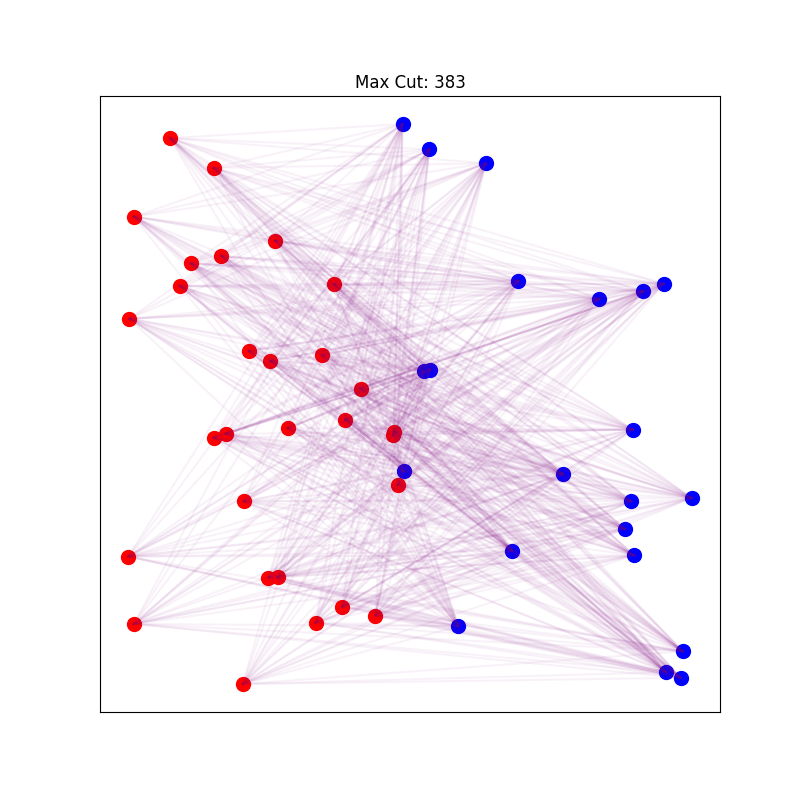
\includegraphics[scale=.5]{assets/max-cut-solution.png}
  \caption{Set 1 is red and Set 2 is blue. Cut edges are given in purple. There is an edge between ever pair of vertices but only cut edges are shown.}
\end{figure}

\subsubsection{Extra Credit}
\begin{itemize}
\item\label{item:1} The SDP problem that we formulated was an approximation for the max-cut problem - not the optimal solution. If we were able to set \( x_{i, j} \in \{ -1, 1 \} \) then we would have an optimal solution. We will try and see how well the SDP solver did:
\item\label{item:2}
Create a brute force max-cut solver and compare the results to what the SDP found.
\item\label{item:3}
Note that such a brute force solver will have a \( O(2^n) \) runtime so be careful for large values of \( n \).
\item\label{item:4}
Using a simulation approach, how well of a bound does the SDP problem set?
\item\label{item:5}
In question 7. we got a potential max-cut. How well does this compare to the actual optimal max-cut?
\end{itemize}



\newpage
\subsection{References}
\begin{thebibliography}{12}
% \item\url{https://users.math.msu.edu/users/iwenmark/Teaching/MTH995/Papers/SDP_notes_Marina_Epelman_UM.pdf}
\bibitem{Arora} 1.Arora S, Hazan E, Kale S. Fast Algorithms for Approximate Semidefinite Programming using the Multiplicative Weights Update Method \url{https://www.cs.princeton.edu/~arora/pubs/mw-focs.pdf}
\bibitem{Candes} 1.Candès E, Recht B. Exact matrix completion via convex optimization. Communications of the ACM. 2012;55(6):111-119. doi:\url{https://doi.org/10.1145/2184319.2184343}
\bibitem{Myo} Myo W. A Real Life Application of Linear Programming. 2012;4. \url{https://www.uit.edu.mm/storage/2020/09/WWM-2.pdf}
\bibitem{Zhou} Zhou X, Yang C, Zhao H, Yu W. Low-Rank Modeling and Its Applications in Image Analysis. ACM Computing Surveys. 2014;47(2):1-33. doi:\url{https://doi.org/10.1145/2674559}
‌
\end{thebibliography}

\end{document}
